\chapter{Groundbreaking Inventions in Information and Communication Technology}

%~ \centerline{{\LARGE\sl Understanding IP Routing}}
\vskip -12pt

\centerline{{\LARGE Talk at the Book Launch Function}}

\vskip 0.8cm

\begin{center}
{\large\uppercase{$\text{Srinivasan Ramani}$}} 


\vskip -6pt

\end{center}

\vskip 2cm




\vfill




\newpage

\begin{multicols}{2}

Why do I call “Groundbreaking Inventions in ICT” a great book? Firstly, because it deals with a very important topic – the revolution that changed our lives. \textbf{The book helps us celebrate the IT revolution}. The last fifty or sixty years have been a great time. Something similar to the Industrial Revolution. However, everyone did not recognize what was happening in the early years of the revolution. I had asked my college principal to be allowed to change to another college so that I could study electronics. He did not allow me to do that. “First complete the BE in electrical engineering you are doing”, he said, “then you can be sure of a job. With electronics and all that, who knows? You might be hunting for a job!” He gave me a concession though; “You can do a master’s degree course in electronics after your BE, if you want to!”

\vspace{-.1cm}

Let us talk about economic growth. I will borrow some statistics from sources other than Professor’s book. The World (nominal) GDP has gone up from roughly 11 Trn to 80 Trn \$ over the last 60 years. It has grown faster than the world population. Researchers estimate that “the digital economy is worth \$11.5 trillion globally, equivalent to 15.5 percent of global GDP and has grown two and a half times faster than global GDP over the past 15 years.” Compare this with the contribution of the Agriculture Sector (4\%) to the world GDP as reported in World Development Indicators: Structure of output \cite{art3-key01} by the World Bank group. In which year was this the case? Take your pick. It was 4\% in 2010. It was 4\% in 2019. Compare that with the IT Sector.

\vspace{-.1cm}

What made the difference to the poor students of electronics and computer science who had missed the good advice from my Principal?

\vspace{-.1cm}

Much of the difference was due to the fifteen great ideas that this book describes. 

\vspace{-.1cm}

The growth I refer to did not leave India behind. India was the tenth ranker in the world in terms of GDP in 1960. By 2019 it had moved to the $5^{\rm th}$ rank. Where has the growth come from?  And was the growth supported by IT – did it help only the electronics and computer science graduates? Of course not! The benefits have been fairly well spread out.

There is something special about information technology. All along the world has been understood in terms of space and time, matter and energy. The recognition that information is another essential entity was a great step forward. Much of science had been natural science. The rise of the sciences of the artificial has been a major step forward too. \textbf{The book helps us understand the key ideas in information technology.} The selection of ideas has been obviously difficult. Some great ideas have been set aside for the successor to the book. Medical imaging, speech recognition, face recognition, natural language processing, for example. 

I get reminded of the saying that the engineer is the guy who knows how to get things done, and the manager is the guy who tells engineers what to get done. My former boss Mr.~N Vittal, at that time Secretary to Govt in the Dept. of Electronics, used to be asked “Aap electronics engineer hain kya?”. Mr.~Vittal’s answer used to be “Nahi. Hum Electronic Engineer ka Baap hain!” He would explain that his son was an electronics engineer! \textbf{Prof Rajaraman’s book deals with the things that managers understand and value in addition to the technical stuff.}

Great institutions do things in style. They have high standards and confidence in acting as per these standards. Prof. Rajaraman tells the story of a young man at Harvard who is getting ready to receive his Ph.D. The date is set, the family has been informed. He has been offered a job and has accepted it, but his thesis advisory committee rejected his thesis at the last minute. The young man calls his boss on the west coast and says, “My Committee has failed me saying “mostly implementation, not enough maths. The manager says “Join us anyway, and complete your work here adding what they want”. The manager was at Xerox Park at Palo Alto and the young man was Bob Metcalfe, one of the inventors of Ethernet.

Then there is the story of a couple of students who decide to drop out before getting their degree. Their professor encourages them, putting some of his own money into their start-up which grows up in time to be world’s largest Internet company with a market cap of 741 Billion \$. By the way, says Prof. Rajaraman, the Professor concerned had been a graduate of the first batch of the Computer Science Dept. of IIT Kanpur! The Institution from which the students had dropped out was Stanford!  These stories are merely two examples. There are many more in the book. \textbf{We learn as much from these stories as we do from the technical ideas.}

I will conclude by saying that this book is a rare one of its genre. The rarity of such books is one reason that we in the engineering community do not read as much as we should. Our scientific colleagues are much better off. There are so many books on the history of science.  That reminds me of the time I was in the selection committee to identify a Vice President for an IT company. I asked a candidate if he could name a good book he had read in the past year. He looked puzzled and worried. Then he managed to name a book – it was MySQL Reference Manual! That raises the question of what is a good book! Then we can ask what is a great book!

Now you know. \raisebox{-.1cm}{
\includegraphics[scale=.9]{src/Figures/circledC.eps}}

\begin{thebibliography}{99}

\bibitem{art3-key01} \underline{World Development Indicators: Structure of output}, from the World Bank Group.

\bibitem{art3-key02} Huawei \& Oxford Economics. (2017). \textit{Digital Spillover. Measuring the true impact of the Digital Economy}. Retrieved from

\url{ https://www.huawei.com/minisite/gci/en/digital-spillover/files/gci_digital_spillover.pdf}

Quoted by Brookings Institution in

\url{https://www.brookings.edu/research/trends-in-the-information-technology-sector/}

\end{thebibliography}

  
\end{multicols}

\noindent
\begin{tabular}{V{2.5}cp{15.2cm}V{2.5}}
\clineB{1-2}{2.5}
 &\\
\raisebox{-3.3cm}{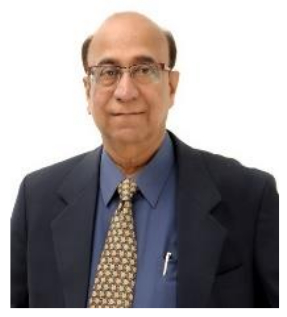
\includegraphics{src/Figures/fig002.jpg}} & 

\centerline{\large\bf Srinivasan Ramani}

\bigskip
Dr. Ramani was Research Director, HP Labs India, located in Bangalore. He founded the National Centre for Software Technology (NCST) in 1985, and had directed it during 1985-2000. His work at NCST covered R \& D in the areas of computer networks and knowledge based computer systems. He made significant contributions to the creation and development of the Indian academic network, ERNET, which brought Internet connectivity to India in 1988, and the Bombay Library Network, Bonet. He has served as Editor, Journal of Information Technology for Development, for a number of years.\\

&\smallskip
He was President, International Council for Computer Communication, and Chairman of the Governing Board of the Information Library Network (INFLIBNET). He was also a member of the High Level Panel of Advisors to the UN on Information and Communication Technologies.\\
&\\ 
\clineB{1-2}{2.5}
\end{tabular}


